\documentclass[bare_jrnl_transmag]{subfiles}
\begin{document}
\subsection{Drone Pose Estimation}
The drone pose estimation from the IMU is required to be accurate for the purposes of the VIO algorithm. Evaluation of the Madgwick filter was performed by comparing the ground-truth pose of the drone to the pose estimated by the Madgwick filter for the validation dataset. The results of the evaluation are shown in Figure \ref{fig:madgwick_results}.

\begin{figure}[H]
    \centering
    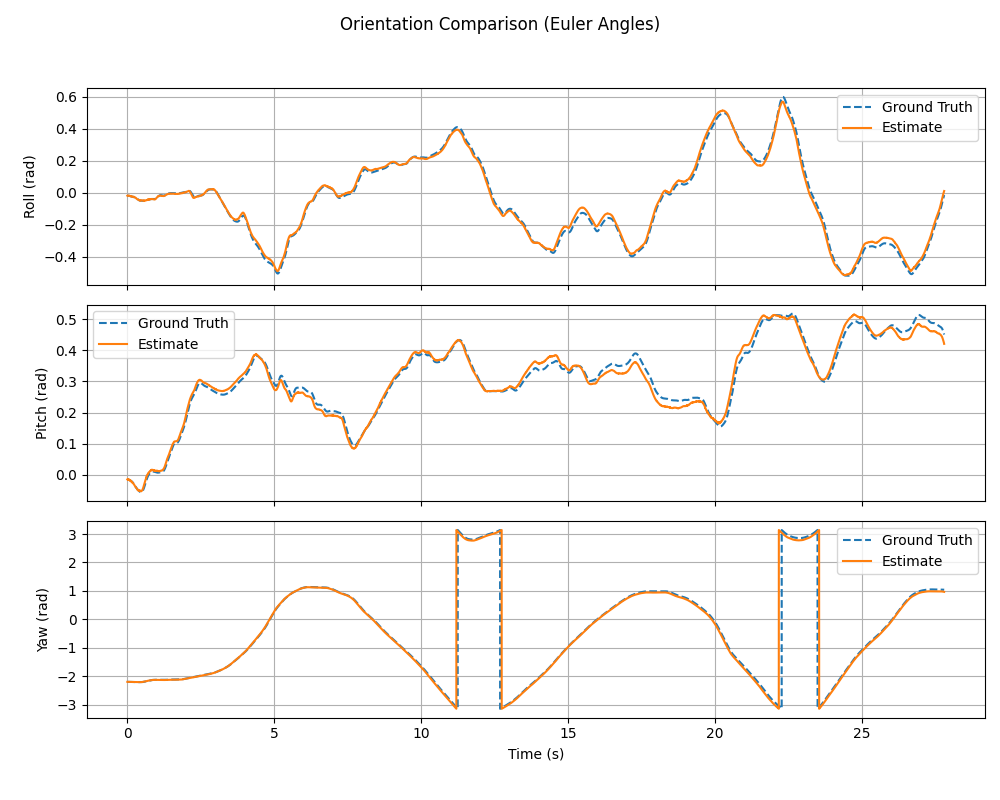
\includegraphics[width=0.8\linewidth]{figures/madgwick_results.png}
    \caption{Madgwick filter results comparing the ground-truth pose of the drone to the pose estimated by the Madgwick filter.}
    \label{fig:madgwick_results}
\end{figure}

The results show that the Madgwick filter is able to estimate the pose of the drone with a high degree of accuracy (RMSE (Roll, Pitch, Yaw): [0.0198 0.0160 0.0425] rad) in real-time, making it suitable for use in the VIO algorithm.

\end{document}